\newpage
\section{APPENDIX}
\begin{comment}
\subsection{Structures Used by Our Algorithm}
\begin{lstlisting}[caption={Data structures used by our algorithm},label=list:struct,numbers=none,keywords={}]
struct WordDescriptor {
    void* address;
    uintptr_t old;
    uintptr_t new;
    MCASDescriptor* parent;
};

enum StatusType { ACTIVE, SUCCESSFUL, FAILED };

struct MCASDescriptor {
    StatusType status;
    size_t N;
    WordDescriptor words[N];
};
\end{lstlisting}
\end{comment}

\subsection{Replacing RDCSS with CAS in Harris et al. algorithm leads to ABA}\label{sec:aba-harris}

Consider two memory locations $a_1$ and $a_2$ with initial values $v_1$ and $v_2$ respectively. Consider two $2$-\cas{} operations $op$ and $op'$ which operate on $a_1$ and $a_2$. $op$ has old values $v_1$ and $v_2$ and new values $v_1'$ and $v_2'$, respectively; $op'$ has old values $v_1'$ and $v_2'$ and new values $v_1$ and $v_2$, respectively. Let $D$ be $op$'s descriptor.

\begin{enumerate}
    \item $op$ executes solo and performs the \cas{} to make $a_1$ point to $D$, then pauses immediately before the \cas{} to acquire $a_2$.
    \item $op'$ executes solo: it first helps $op$ complete, changing the values of $a_1$ and $a_2$ to $v_1'$ and $v_2'$ respectively; then $op'$ performs its own changes, modifying $a_1$'s and $a_2$'s values back to $v_1$ and $v_2$, respectively. 
    \item $op$ resumes, successfully acquires $a_2$, performs the status-change \cas{} on $D$, then performs unlocking \cas{}es on $a_1$ and $a_2$. The \cas{} on $a_1$ will fail, and $a_1$'s value will remain $v_1$. The \cas{} on $a_2$ will succeed, changing its value to $v_2'$.
    \item The values of $a_1$ and $a_2$ are now incompatible with any linearization of $op$ and $op'$.
\end{enumerate}

\subsection{Correctness of Volatile \texorpdfstring{$k+1$}{k+1} algorithm}
\label{sec:appendix-correctness}
\label{sec:k+1-mcas-correctness}
In this section we argue that our \mcas{} algorithm is linearizable and lock-free. We give preliminary invariants before showing the main results. 
% Due to space constraints, some proofs have been moved to the optional appendix. 
% fAll line references refer to Listing~\ref{list:algo} unless otherwise specified.

\begin{lemma}\label{finalized-status}
    Once an \mcas{} descriptor is finalized, its status never changes again. \normalfont{The status can only be modified through the \cas{} at Line~\ref{mcas-finalize}, whose expected value is \ttactive. If the \cas{} succeeds, the new value of the status can only be \successful\ or \failed, thus any subsequent attempt to change the status will fail.}
\end{lemma}

\begin{lemma}
    An \mcas{} descriptor is finalized by at most one thread. \normalfont{This follows from the fact that a descriptor is finalized through a \cas{} and the fact that an \mcas{} descriptor cannot change status after being finalized (Lemma~\ref{finalized-status})}.
\end{lemma}


\begin{lemma}
    If at least one thread attempts to finalize a descriptor $d$, some thread will successfully finalize $d$. \normalfont{The initial status of a descriptor is \ttactive. Any thread attempting to finalize a descriptor does so through the CAS at Line~\ref{mcas-finalize}, with expected value \ttactive. Thus, at least one CAS finds the status to be \ttactive\ and successfully changes it.}
\end{lemma}

\begin{lemma}\label{finalized-successful}
    An \mcas{} descriptor $d$ is finalized as successful only if some thread observed all target locations of $d$ to be acquired by $d$. \normalfont{This is because the status is changed to successful only if the \texttt{success} variable is true at Line~\ref{mcas-finalize}. This only happens if some thread completed the for-loop over all of $d$'s {\worddescriptor}s without exiting the loop at Line~\ref{for-break}. The only two ways for a thread to move to the next \worddescriptor\ in the loop is if the thread sees the current target location was already acquired by $d$ (Line~\ref{disregarded}) or if the thread successfully acquired the current target location for $d$ (Line~\ref{mcas-acquire}). In both cases the thread observed the target location to be acquired by $d$.}
\end{lemma}
 
\begin{lemma}\label{finalized-failed}
    An \mcas{} descriptor $d$ is finalized as failed only if some thread observed a target location of $d$ to contain a different value than its expected value in $d$. \normalfont{This is because the only way for the status to be changed to failed is if the \texttt{success} variable is false. This only happens if some thread observed the current value of a target location is different from its expected value in Line~\ref{doomed-start}.}
\end{lemma}

\begin{lemma}\label{lemma-acquired-forever}
    After a location $l$ becomes acquired by some operation $op$, $l$ will never become un-acquired again. \normalfont{This is because the only instruction that modifies a location $l$ is the acquire \cas{} at Line~\ref{mcas-acquire}.}
\end{lemma}

We say that an operation $op_1$ {\em helps} an \mcas{} operation $op_2$ if $op_1$ calls \mcas{} with $op_2$'s descriptor in Line~\ref{mcas-help}. 

\begin{lemma}\label{lemma-change-owner}
    After a location $l$ becomes acquired by some operation $op$, no operation $op' \ne op$ will acquire $l$ before $op$ becomes finalized. \normalfont{Assume by contradiction that $op'$ acquires $l$ after $op$ acquires $l$ and while $op$ is still active. Consider $op'$ last call to \readInternal\ (Line~\ref{mcas-readinternal}) before the successful acquisition of $l$. During this call, $op'$ must have observed that $l$ is owned by $op$ (otherwise; if $op$ had acquired $l$ after the call to \readInternal, the acquisition \cas{} would have failed). Moreover, $op$ was active during that call to \readInternal\ by $op'$. Thus, $op'$ helped $op$ before returning from \readInternal, finalizing $op$ in the process. Thus $op$ cannot be active at the time of the acquisition, a contradiction.}
\end{lemma}

We say that a location $l$ is \textit{re-acquired} by operation $op$ at time $t$ if (1) $l$ becomes acquired by $op$ at time $t$, (2) there exists time $t' < t$ such that $l$ became acquired by $op' \ne op$ at time $t'$, and (3) there exists time $t'' < t'$ such that $l$ became acquired by $op$ at time $t''$.

\begin{lemma}\label{lemma-no-reacquisition}
    A location cannot be re-acquired. 
    \normalfont{ Assume the contrary and let $t$ be the earliest time when any location is re-acquired in a given execution $E$. Let $l$ be that location and $op$ be the operation re-acquiring it. This means that $l$ became acquired by $op$ at some time $t''$, then became acquired by some $op'\ne op$ at time $t' > t$ and then later became acquired by $op$ at time $t > t'$ (the times in this lemma are represented in the figure below, for convenience). By Lemma~\ref{lemma-change-owner}, $op$ must have become finalized at some time $t_f < t'$ ($t_f$ is unique by Lemma~\ref{finalized-status}).
    
    Now consider the thread $T$ which acquires $l$ on behalf of $op$ at time $t$. $T$ does so through the \cas{} at line~\ref{mcas-acquire}. Since $op$ becomes finalized at time $t_f$, $T$ must have performed the status check at line~\ref{status-check} at some time $t_s < t_f$ (otherwise $T$ would have exited from the for loop without acquiring $l$). Let $t_r < t_s$ be the last time when $T$ performed \readInternal{} (line~\ref{mcas-readinternal}) before $t_s$. Note that $t_r < t''$, otherwise $T$ would have seen $l$ as already acquired by $op$ at line~\ref{disregarded} and continued without attempting to acquire $l$.  
    
    Let $\langle c,v \rangle$ be the return value of the \readInternal{} call by $T$ at $t_r$; this means that $l$'s value was $c$ at some time before $t_r$. Since $T$ successfully performs the CAS at line~\ref{mcas-acquire} at time $t$, the value of $l$ must also be $c$ immediately before $t$. However, the acquisition of $l$ at time $t'' > t_r$ changes the value of $l$ from $c$. Therefore, it must be the case that some thread changes the value of $l$ back to $c$ at some time $t_c$ between $t''$ and $t$. Note that $c$ must be a word descriptor (due to Lemma~\ref{lemma-acquired-forever}). Since word descriptors are unique, they uniquely identify their parent operations. Therefore, $l$ must have been owned by some operation $op''$ before $t_r$ and again at $t_c$; this means that $op''$ \textit{re-acquired} $l$ at time $t_c$, contradicting our choice of $t$ as the earliest re-acquisition time.}
    
\end{lemma}

\noindent
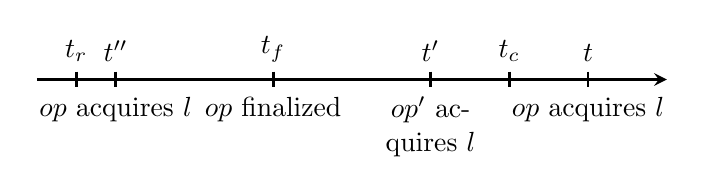
\begin{tikzpicture}
\usetikzlibrary{calc}

% draw arrow
\coordinate (start) at (-4,0);
\coordinate (end) at (4,0);
\draw [line width=1pt, -stealth] (start) -- (end);

% You can use `foreach` to improve the following codes
\coordinate (s0) at (-3,0);
\coordinate (t00) at ($(s0)+(0,0.1)$);
\coordinate (t01) at ($(s0)-(0,0.1)$);
\coordinate (s1) at (1,0);
\coordinate (t10) at ($(s1)+(0,0.1)$);
\coordinate (t11) at ($(s1)-(0,0.1)$);
\coordinate (s2) at (3,0);
\coordinate (t20) at ($(s2)+(0,0.1)$);
\coordinate (t21) at ($(s2)-(0,0.1)$);
\coordinate (s3) at (-1,0);
\coordinate (t30) at ($(s3)+(0,0.1)$);
\coordinate (t31) at ($(s3)-(0,0.1)$);
\coordinate (s4) at (-3.5,0);
\coordinate (t40) at ($(s4)+(0,0.1)$);
\coordinate (t41) at ($(s4)-(0,0.1)$);
\coordinate (s5) at (2,0);
\coordinate (t50) at ($(s5)+(0,0.1)$);
\coordinate (t51) at ($(s5)-(0,0.1)$);


% draw ticks
\draw [line width=1pt] (t00) -- (t01);
\node [anchor=south] at (t00.north) {$t''$};

\draw [line width=1pt] (t10) -- (t11);
\node [anchor=south] at (t10.north) {$t'$};

\draw [line width=1pt] (t20) -- (t21);
\node [anchor=south] at (t20.north) {$t$};

\draw [line width=1pt] (t30) -- (t31);
\node [anchor=south] at (t30.north) {$t_f$};

\draw [line width=1pt] (t40) -- (t41);
\node [anchor=south] at (t40.north) {$t_r$};

\draw [line width=1pt] (t50) -- (t51);
\node [anchor=south] at (t50.north) {$t_c$};

% add texts
\node [anchor=north, align=center, text width=2cm] at (t01.south) {
$op$ acquires $l$
};

\node [anchor=north, align=center, text width=2cm] at (t11.south) {
$op'$ acquires $l$
};

\node [anchor=north, align=center, text width=2cm] at (t21.south) {
$op$ acquires $l$
};

\node [anchor=north, align=center, text width=2cm] at (t31.south) {
$op$ finalized
};

\end{tikzpicture}

\begin{lemma}
    A location $l$ cannot be acquired by operation $op$ after $op$ is finalized as successful.
    \normalfont{This follows from Lemmas~\ref{finalized-successful} and \ref{lemma-no-reacquisition}.}
\end{lemma}

% \begin{lemma}
%     When an \mcas{} operation $op$ attempts to acquire location $l$, then all of $op$'s target locations up to $l$ in the sorting order are already owned by $op$. \normalfont{This is because we assume that $op$'s {\worddescriptor}s are in sorted order and $op$ iterates through them one by one, without continuing to the next location if the current location was not acquired.} 
% \end{lemma}
% \begin{lemma}\label{lemma-helping-finalized}
%     If, at time $t$, $op_1$ is helping $op_2$ and $op_1$ is finalized, then $op_2$ is also finalized at time $t$. \normalfont{This is because operations first help finalize \mcas{} operations on which they depend, before continuing their own execution.}
% \end{lemma}

\begin{lemma}\label{lemma-higher-highest}
    If $op_1$ helps $op_2$, then either $op_2$ highest acquired location is higher than $op_1$'s highest acquired location, or $op_1$ has not acquired any locations. \normalfont{If $op_1$ is a read operation, the statement is trivially true. Assume now that $op_1$ is an \mcas{} operation that helps $op_2$ and that $op_1$'s highest acquired location is higher than $op_2$'s highest acquired location ($\star$). Since $op_1$ helps $op_2$, $op_1$ has observed one of its target locations $l$ to be already acquired by $op_2$. But since $op_1$ iterates over locations in increasing order, $l$ must be higher than $op_1$'s highest acquired location. This contradicts $\star$.}
\end{lemma}

We define the {\em helping graph at time $t$}, $H(t)$, as follows. The vertices of $H(t)$ are the ongoing operations at time $t$. There is an edge from $op_1$ to $op_2$ if $op_1$ is helping $op_2$ at $t$. We define the {\em call depth} of an operation $op$ at time $t$ to be the length of the longest path starting from $op$ in $H(t)$.
% \begin{lemma}\label{lemma-no-cycle}
%     For any time $t$, $H(t)$ does not contain a cycle.\normalfont{Assume the contrary and let $C$ be a cycle in $H(t)$. $C$ cannot contain any reads, since reads are not helped in our algorithm. 
    
%     We consider two possibilities. (1) $C$ contains a finalized operation $op$. Then, by Lemma~\ref{lemma-helping-finalized}, all operations in $C$ must be finalized. 
    
%     Let $(op, op')$ be the last edge to have been added to $C$. Then, at some time $t'<t$, $op$ must have read $op'$'s status as active at line~\ref{read-internal-check}. }
% \end{lemma}
\begin{lemma}\label{lemma-call-depth}
    For any operation $op$ and any time $t$, the call depth of $op$ at $t$ is finite. \normalfont{Assume the contrary. Since each thread can have at most one ongoing operation at $t$, $H(t)$ has a finite vertex set. Let $op$ be an operation and $t$ be a time such that $op$ has an infinite call depth at $t$. Then, $H(t)$ must contain a cycle. This is a contradiction: if the cycle contains an operation $op_0$ that has no acquired locations, then $op_0$'s predecessor in the cycle cannot be helping it; if the cycle does not contain such an operation, then by traversing the cycle we would find operations with strictly increasing highest acquired locations (Lemma~\ref{lemma-higher-highest}).}
\end{lemma}

Informally, Lemma~\ref{lemma-call-depth} says that while in our algorithm it is possible for operations to recursively help one another, the recursion depth is finite at any time, due to the sorting of memory locations.

We define the following predicates (recall that $n$ is the number of threads). Let $S(k)$: ``If there are $0 < k \leq n$ concurrent operations and at least one thread is taking steps and no operations are created, at least one operation will eventually return''. Let $P(k)$: ``If there are $0 < k \leq n$ concurrent operations and at least one thread is taking steps, at least one operation will eventually return''.

\begin{lemma}\label{sk}
    $S(k)$ is true for all $k$, $0 < k \leq n$. \normalfont{Assume the contrary. Pick an active thread $T$: $T$ is taking steps infinitely often, but no operations ever return. By Lemma~\ref{lemma-call-depth}, the call  depth of $T$ is finite, thus $T$ must be taking some backward branch infinitely often. If $T$ is taking the branch at Line~\ref{read-internal-retry} infinitely often, then \mcas{} operations are being finalized infinitely often (Line~\ref{read-internal-retry} is only executed if some operation was active at Line~\ref{read-internal-check}; but that same operation must be finalized by Line~\ref{read-internal-retry} due to the preceding \mcas{} call which returns only after the operation is finalized). This is a contradiction because we started with a finite number of \mcas{} operations and no operations are being created. If $T$ is taking the branch at Line~\ref{mcas-retry} infinitely often, then locations either (a) become acquired infinitely often or (b) change owners infinitely often. Both possibilities lead to a contradiction: (a) because there are a finite number of target locations of ongoing \mcas{} operation and locations never become unacquired and (b) because locations change owners only after operations become finalized, which would imply that operations become finalized infinitely often.}
\end{lemma}

\begin{lemma}\label{lemma-pk}
    $P(k)$ is true for all $k$, $0 < k \leq n$. \normalfont{Consider the case $k=n$. $P(k)$ is equivalent to $S(k)$ in this case (no operations can be created if there are already as many operations as threads), and thus true. Consider the case $k = n-1$. If some operation is eventually created, then eventually some operation will return, by $P(n)$. If no operation is ever created, then eventually some operation will return, by $S(n-1)$. We can continue in this manner with $k=n-2,...,1$, each time using either $P(k+1)$ or $S(k)$.}
\end{lemma}

\begin{lemma}
    Our implementation is lock-free. \normalfont{This follows immediately from Lemma~\ref{lemma-pk}.}
\end{lemma}

\begin{lemma}
    Linearization point of a failed \mcas{}. \normalfont{By Lemma~\ref{finalized-failed}, if descriptor $d$ is finalized as failed by thread $T$ at time $t_1$, then at time $t_0 < t_1$, $T$ has observed some target location $l$ to contain a different value than $l$'s expected value in $d$. We can take $t_0$ as the linearization point of the \mcas{}.}
\end{lemma}


\begin{lemma}
    Linearization point of a successful \mcas{}. \normalfont{By Lemma~\ref{finalized-successful}, if thread $T$ changes the status of descriptor $d$ to successful, then $T$ previously observed all of $d$'s target locations to be acquired by $d$. Thus, when changing the status of $d$ to successful, $T$ changes the logical values of all target locations, marking the linearization point.}
\end{lemma}

\begin{lemma}
    Linearization point of a read. \normalfont{The linearization point of a read is the last executed dereference instruction at Line~\ref{read-internal-first-read}.} 
\end{lemma}

\subsection{Persistent \mcas{} with \texorpdfstring{$k+1$}{k+1} \cas{} and 2 Persistent Fences}\label{app:persistent-mcas}
\bigskip
\begin{lstlisting}[caption={[Our \mcas{} algorithm for persistent memory.]Our \mcas{} algorithm for persistent memory. Commands in {\it italic} are related to memory reclamation, and \uline{underlined} commands are related to persistence.},label=list:algo-persistent,firstnumber=1,keywords={}]
read(void* address) { @\label{pread_begin}@
    @{\it epochStart();}@@\label{pread-epoch-start}@
    <content, value> = readInternal(address, NULL);@\label{pread-line2}@
    @{\it epochEnd();}@@\label{pread-epoch-end}@
    return value; } @\label{pread_end}@

MCAS(MCASDescriptor* desc) {
    @{\it epochStart();}@
    success = true;
    for wordDesc in desc->words {@\label{pmcas-first-phase-begin}@
retry_word:
        <content, value> = readInternal(wordDesc.address, desc); @\label{pmcas-readinternal}@
        // if this word already points to the right place, move on
        if (content == &wordDesc) continue;@\label{pdisregarded}@
        // if the expected value is different, the MCAS fails
        if (value != wordDesc.old) {@\label{pdoomed-start}@ success = false; break; @\label{pfor-break}@ }@\label{pdoomed-end}@
        if (desc->status != ACTIVE) break; @\label{pstatus-check}@
        // try to install the pointer to my descriptor; if failed,    retry
        if (!CAS(wordDesc.address, content, &wordDesc)) @\label{pmcas-acquire}@goto retry_word;@\label{pmcas-retry}@ }@\label{pmcas-first-phase-end}@
    @\uline{for wordDesc in desc->words \{ PERSISTENT\_FLUSH(wordDesc.address); \}}@
    @\uline{PERSISTENT\_FENCE();}\label{fence-acquire}@
    newStatus = success ? SUCCESSFUL : FAILED;
    if (CAS(&desc.status, ACTIVE, newStatus @\uline{| DirtyFlag}@)){@\label{pmcas-finalize}@
        // if I finalized this descriptor, mark it for reclamation
        @{\it retireForCleanup(desc);}@@\label{pretire-for-cleanup}@ }@\label{pmcas-finalize-end}@
    @\uline{PERSISTENT\_FLUSH(\&desc.status);}@
    @\uline{PERSISTENT\_FENCE();}\label{fence-finalize}@
    @\uline{parent->status = parent->status \& \textasciitilde{}DirtyFlag;}@ @\label{unset-dirty}@
    returnValue = (desc.status == SUCCESSFUL);
    @{\it epochEnd();}@
    return returnValue; }
\end{lstlisting}
\newpage
\begin{lstlisting}[caption={[The \readInternal\ auxiliary function, used by our \mcas{} algorithm for persistent memory.]The \readInternal\ auxiliary function, used by our \mcas{} algorithm for persistent memory. \uline{Underlined} commands are related to persistence.},label=list:readInternal-persistent,keywords={},firstnumber=last]
readInternal(void* addr, MCASDescriptor *self) {@\label{pr_i_begin}@
retry_read:                            
    val = *addr;@\label{pread-internal-first-read}@
    if (!isDescriptor(val))@\label{pread-internal-line4}@ then return <val,val>;@\label{pread-internal-line5}@
    else { // found a descriptor@\label{pread-internal-line6}@
        MCASDescriptor* parent = val->parent;@\label{pread-internal-line7}@
        if (parent != self) && parent->status == ACTIVE) {@\label{pread-internal-check}@
            MCAS(parent);@\label{pmcas-help}@
            goto retry_read; @\label{pread-internal-retry}@
        @\uline{\} else if (parent->status \& DirtyFlag) \{}@
            @\uline{PERSISTENT\_FLUSH(\&parent->status);}@
            @\uline{PERSISTENT\_FENCE();}@
            @\uline{parent->status = parent->status \& \textasciitilde{}DirtyFlag;}@
            @\uline{goto retry\_read;}@
        } else {@\label{pread-internal-line11}@
            return parent->status == SUCCESSFUL ?
                <val,val->new> : <val,val->old>;@\label{pread-internal-line12}@
}  }  }@\label{pr_i_end}@
\end{lstlisting}

\subsection{Memory Management}
\label{sec:mem-mgt-app}
We describe the memory management in the context of the \mcas\ implementation presented in Section~\ref{sec:algos}.
% and mention the required changes to support the optimal algorithm presented in Section~\ref{sec:optimality} at the end of this section.

We use two thread-local lists for reclaiming operation descriptors:
One list is for descriptors that have been finalized, but not detached yet (\texttt{finalizedDescList}), and another is for
descriptors that have been detached but to which readers might still hold references (\texttt{detachedDescList}).

In general, our memory management scheme is similar to an RCU (read-copy-update) implementation~\cite{McKenney17, MS98}.
We start with a simple blocking scheme, extending it into a non-blocking one.
Each thread maintains an epoch number, incremented by the thread 
upon the entry to and before the exit from the \ttread\ and \mcas\ functions
(see, e.g., Lines~\ref{read-epoch-start} and~\ref{read-epoch-end} in Listing~\ref{list:algo}).
In \texttt{retireForCleanup} function (cf.\ Line~\ref{retire-for-cleanup} in Listing~\ref{list:algo}), a thread adds the given descriptor 
to \texttt{finalizedDescList}.
Once the size of this list reaches a certain threshold, the thread invokes a function similar semantically to \texttt{synchronize\_rcu()}~\cite{McKenney17}.
That is, it runs through all thread epochs, and waits for every epoch with an odd value (indicating that a thread
is inside the \ttread\ or \mcas\ functions) to advance.
Once all epochs are traversed, all descriptors currently in the \texttt{detachedDescList} list can be 
reclaimed (returned to the operating system or put into a list of available descriptors for reuse).
At the same time, all descriptors currently in the \texttt{finalizedDescList} list can be moved
to the \texttt{detachedDescList} list, after replacing pointers to those descriptors in corresponding memory locations with their actual values.

To elaborate on this last step, given an \texttt{MCASDescriptor} descriptor \texttt{d} that is about to be moved 
from \texttt{finalizedDescList} to \texttt{detachedDescList},
a thread runs through all the \texttt{WordDescriptor}s stored in \texttt{d}.
For every such \texttt{WordDescriptor} \texttt{w}, the thread checks whether \texttt{w->address} is equal to \texttt{d} and if so,
writes \texttt{w->old} or \texttt{w->new} into \texttt{w->address} according to the status of \texttt{d}.
The check and the write are done atomically using \cas{}.

The scheme presented so far is blocking---if a thread does not advance its epoch number, any thread will be unable 
to complete the traversal of epochs.
To avoid this issue, each thread may store a local copy of all thread epochs it has seen during the last traversal.
On its next epoch traversal, it compares the current and the previously seen epochs for each thread $t$, and if those
two are different, it infers that $t$ has made progress.
If progress is detected for all threads, 
any descriptor that was placed into \texttt{finalizedDescList} (\texttt{detachedDescList}) before 
the previous epoch traversal can be detached (reclaimed, respectively).

Note that while this scheme is non-blocking, a failure of a thread might prevent reclamation of \emph{any} memory associated with descriptors.
This is a common issue with epoch-based reclamation schemes~\cite{DHK16}, which could be resolved either by 
enhancing the scheme (e.g., as in~\cite{Brown15}) or by switching to a different scheme, e.g., one based on hazard pointers~\cite{DHK16,Michael04}.

% The optimal \mcas\ algorithm in Section~\ref{sec:optimality} requires a few modifications to the memory management scheme presented so far. First, since that algorithm does not use a \code{status} field, a call to \texttt{retireForCleanup} is done by a thread that ``locks'' the last word (if the corresponding \mcas\ operation is successful) or installs a pointer to the failure descriptor (if not). Second, we need to ensure that the status of an applied \mcas\ operation is known (to any thread that may read a pointer to the descriptor of that operation) while the corresponding descriptor is being recycled. Otherwise, a thread may try to help an already applied operation. To that end, we reintroduce the \texttt{status} field into the operation descriptor. This field is set (with a simple store) in \texttt{retireForCleanup}, \emph{before} any of the pointers to the descriptor is detached. Any thread that finds a pointer to a descriptor (in \texttt{readInternal}) checks the \texttt{status} field before deciding to help the corresponding \mcas\ operation (i.e., exactly as shown in Listing~\ref{list:readInternal}). Finally, we note that when persistence is considered, setting the status of an operation in \texttt{retireForCleanup} has to be followed by a persistent fence. This fence, however, can be aggregated over all operation descriptors that are about to be recycled, and nevertheless takes place off the critical path.

\subsection{Managing Persistent Memory}
\label{sec:persistent-memory}
In this section, we show how the memory management mechanism described in Section~\ref{sec:mem-mgmt} is extended to manage persistent memory.
Upon recovery from a crash, any pending \pmcas\ operation is applied using the same algorithm as presented in Listing~\ref{list:algo}.
Pending \pmcas\ operations can be found by scanning allocated descriptors (e.g., if descriptors are allocated from a pool, similar to David et al.~\cite{david18}).
Moreover, since we assume the recovery is done by a single thread, we can immediately 
detach and recycle any finalized descriptor (after writing back the actual values into corresponding memory locations).
Therefore, when considering persistent memory, 
the only change required to support correct recycling of descriptors (in addition to using a persistent memory allocator) is
flushing all writes while detaching descriptors and introducing a persistent fence 
right before reclaiming descriptors from \texttt{detachedDescList}.
The fence is required to avoid a situation where a detached descriptor is recycled and a crash happens while 
the descriptor is being initialized with new values.
In this case, and if a fence is not used, 
some memory locations may still point to the descriptor (since updates to those locations might have not been persisted before the crash), 
while the descriptor may already be updated with new content.
Note, though, that the flushes and the fence take place off the critical path, 
therefore their impact on the performance of \pmcas\ is expected to be negligible.


\subsection{Efficient Reads}
\label{sec:reads}
Once a memory location has been modified by an \mcas\ operation, even if by a failed one, it would
refer to an operation descriptor until that descriptor is detached.
Until that happens, the latency of a read operation from that memory location would be increased as it would have to access  
an operation descriptor to determine the value that needs to be returned by the read.
The memory management mechanism as described above, however, would detach the descriptor only
as a part of an \mcas\ operation.
This might cause degraded performance for read-dominated workloads in which \mcas\ operations are rare.

To this end, we propose the following optimization for eventual removal of references to an operation descriptor 
and storing the corresponding value directly in the memory location as part of the read operation.
If a read operation finds a pointer to a finalized operation descriptor, it will generate a pseudo-random number\footnote{Generating 
a local pseudo-random number is a relatively inexpensive operation that requires only a few processor cycles (see, for instance, the generator in ASCYLIB~\cite{ascylibcode}.)}.
With a small probability, it will run a simplified version of the memory reclamation scheme described above.
Specifically, it will scan epochs of all other threads, and then change the contents of the memory location it attempts to read
to the actual value (using \cas{}).
(To avoid deadlock between two threads scanning epoch numbers, a thread may indicate that it is in the middle of an epoch scan
so that any descriptor can be detached, but not recycled at that time.)

\subsection{Performance in read- and update-heavy workloads}\label{sec:extra-evaluation}

Figures~\ref{fig:dll-appendix} and \ref{fig:btree-appendix} show performance results for the 50\%, 98\%, and 100\% reads workloads in the doubly-linked list and B+-tree benchmarks, respectively. All other settings are the same as in Section~\ref{sec:eval}.
These more extreme workloads largely magnify the performance effects demonstrated by the workloads included in the paper (see Section~\ref{sec:eval}). Namely, as the write ratio increases, so does the gap by which AOPT outperforms PMwCAS in cases that involve contention between concurrent \mcas{} operations (i.e., small and moderate lists and trees). With 100\% reads, our algorithm performs on par with or slightly trails behind PMwCAS at every contention level. Since the workload involves no update operations (and thus no \mcas{}es), the lower complexity of our \mcas{} operations does not factor into the results, whereas the higher overhead of the extra-level of indirection in our read operations does factor in. %To better illustrate the slowdown effect of indirection on our read operations, we also measure the performance of an unsafe (incorrect) version of our algorithm (labeled \textit{AOPT-unsafe} in Figure~\ref{fig:dll}). In this unsafe version, an \mcas{} descriptor is detached immediately after the corresponding \mcas{} operation is applied. This is safe only if an \mcas{} operation is not helped by other concurrent threads. This guarantee is provided in the read-only workload, as the list is initialized by one (main) thread during the warm-up phase. The latter is followed by the actual benchmarking phase in which threads do not apply any \mcas{} operations. We note that in \textit{AOPT-unsafe}, reads do not need to go through an extra layer of indirection and can read values directly from their target locations. As the bottom row of Figure~\ref{fig:dll} shows, eliminating the extra level of indirection brings the performance of AOPT-unsafe in line with the performance of PMwCAS.
% With 100\% reads, PMwCAS outperforms our algorithm at every contention level, because of the extra level of indirection of our reads. This is further confirmed by the \textit{AOPT-unsafe} version of our algorithm, which does not suffer from the extra level of indirection and performs virtually identically to PMwCAS.

\begin{figure*}
\centering
\begin{tikzpicture}
	
    \begin{groupplot}[
        group style=    {group name=my plots,
                        group size=3 by 3,
                        horizontal sep=0.7cm,
                        vertical sep=1.3cm},
        height=3.6cm,
        width=5.2cm,
        ytick scale label code/.code={},
        legend columns=-1,
        xlabel={Number of Threads},
    ]
        
    % Row 1
    \nextgroupplot[
        ylabel = {Throughput (Mops/s)},
        legend entries={AOPT,PMWCAS},
        legend to name=CommonLegend4,    
    ]
    \addplot table[x=Threads,y=AOPT] {data/dl-list/dl-list-list_size-5-search_pct-50-absolute-perf.log};
    \addplot table[x=Threads,y=PMWCAS] {data/dl-list/dl-list-list_size-5-search_pct-50-absolute-perf.log};
    \nextgroupplot
    \addplot table[x=Threads,y=AOPT] {data/dl-list/dl-list-list_size-50-search_pct-50-absolute-perf.log};
    \addplot table[x=Threads,y=PMWCAS] {data/dl-list/dl-list-list_size-50-search_pct-50-absolute-perf.log};
    \nextgroupplot
    \addplot table[x=Threads,y=AOPT] {data/dl-list/dl-list-list_size-500-search_pct-50-absolute-perf.log};
    \addplot table[x=Threads,y=PMWCAS] {data/dl-list/dl-list-list_size-500-search_pct-50-absolute-perf.log};
    
    % Row 2
    \nextgroupplot[ylabel = {Throughput (Mops/s)}]
    \addplot table[x=Threads,y=AOPT] {data/dl-list/dl-list-list_size-5-search_pct-98-absolute-perf.log};
    \addplot table[x=Threads,y=PMWCAS] {data/dl-list/dl-list-list_size-5-search_pct-98-absolute-perf.log};
    \nextgroupplot
    \addplot table[x=Threads,y=AOPT] {data/dl-list/dl-list-list_size-50-search_pct-98-absolute-perf.log};
    \addplot table[x=Threads,y=PMWCAS] {data/dl-list/dl-list-list_size-50-search_pct-98-absolute-perf.log};
    \nextgroupplot
    \addplot table[x=Threads,y=AOPT] {data/dl-list/dl-list-list_size-500-search_pct-98-absolute-perf.log};
    \addplot table[x=Threads,y=PMWCAS] {data/dl-list/dl-list-list_size-500-search_pct-98-absolute-perf.log};  
    
    % Row 3
    \nextgroupplot[ylabel = {Throughput (Mops/s)}]
    \addplot table[x=Threads,y=AOPT] {data/dl-list/dl-list-list_size-5-search_pct-100-absolute-perf.log};
    \addplot table[x=Threads,y=PMWCAS] {data/dl-list/dl-list-list_size-5-search_pct-100-absolute-perf.log};
    % \addplot table[x=Threads,y=AOPT-unsafe] {data/dl-list/dl-list-list_size-5-search_pct-100-absolute-perf.log};
    \nextgroupplot
    \addplot table[x=Threads,y=AOPT] {data/dl-list/dl-list-list_size-50-search_pct-100-absolute-perf.log};
    \addplot table[x=Threads,y=PMWCAS] {data/dl-list/dl-list-list_size-50-search_pct-100-absolute-perf.log};
    % \addplot table[x=Threads,y=AOPT-unsafe] {data/dl-list/dl-list-list_size-50-search_pct-100-absolute-perf.log};
    \nextgroupplot
    \addplot table[x=Threads,y=AOPT] {data/dl-list/dl-list-list_size-500-search_pct-100-absolute-perf.log};
    \addplot table[x=Threads,y=PMWCAS] {data/dl-list/dl-list-list_size-500-search_pct-100-absolute-perf.log};
    % \addplot table[x=Threads,y=AOPT-unsafe] {data/dl-list/dl-list-list_size-500-search_pct-100-absolute-perf.log};
    
    \end{groupplot}
	
	\node[anchor=south,rotate=90,yshift=1.2cm] at ($(my plots c1r1.west)$){{\Large\bf 50\% Reads}};
	\node[anchor=south,rotate=90,yshift=1.2cm] at ($(my plots c1r2.west)$){{\Large\bf 98\% Reads}};
	\node[anchor=south,rotate=90,yshift=1.2cm] at ($(my plots c1r3.west)$){{\Large\bf 100\% Reads}};

    \node[anchor=south,yshift=0.2cm] at ($(my plots c1r1.north)$){\Large \bf List Size 5};
    \node[anchor=south,yshift=0.2cm] at ($(my plots c2r1.north)$){\Large \bf List Size 50};
    \node[anchor=south,yshift=0.2cm] at ($(my plots c3r1.north)$){\Large \bf List Size 500};


% 	\end{axis}
\end{tikzpicture}
\\

\ref{CommonLegend4}
\caption{Doubly-linked list benchmark. Top row shows results for 50\% reads workload; middle row shows results for 98\% reads workload; bottom row shows results for 100\% reads workload. Each column corresponds to a different initial list size (5, 50 and 500 elements, respectively).}
\label{fig:dll-appendix}
\end{figure*}

\begin{figure*}
\centering
\begin{tikzpicture}
	
    \begin{groupplot}[
        group style=    {group name=my plots,
                        group size=3 by 3,
                        horizontal sep=0.7cm,
                        vertical sep=1.3cm},
        height=3.6cm,
        width=5.2cm,
        ytick scale label code/.code={},
        legend columns=-1,
        xlabel={Number of Threads},
    ]
        
    % Row 1
    \nextgroupplot[
        ylabel = {Throughput (Mops/s)},
        legend entries={AOPT,PMWCAS},
        legend to name=CommonLegend5,
    ]
    \addplot table[x=Threads,y=AOPT] {data/bztree/bztree-tree_size-16-search_pct-50-absolute-perf.log};
    \addplot table[x=Threads,y=PMWCAS] {data/bztree/bztree-tree_size-16-search_pct-50-absolute-perf.log};
    \nextgroupplot
    \addplot table[x=Threads,y=AOPT] {data/bztree/bztree-tree_size-512-search_pct-50-absolute-perf.log};
    \addplot table[x=Threads,y=PMWCAS] {data/bztree/bztree-tree_size-512-search_pct-50-absolute-perf.log};
    \nextgroupplot
    \addplot table[x=Threads,y=AOPT] {data/bztree/bztree-tree_size-4000000-search_pct-50-absolute-perf.log};
    \addplot table[x=Threads,y=PMWCAS] {data/bztree/bztree-tree_size-4000000-search_pct-50-absolute-perf.log};
    
    % Row 2
    \nextgroupplot[ylabel = {Throughput (Mops/s)}]
    \addplot table[x=Threads,y=AOPT] {data/bztree/bztree-tree_size-16-search_pct-98-absolute-perf.log};
    \addplot table[x=Threads,y=PMWCAS] {data/bztree/bztree-tree_size-16-search_pct-98-absolute-perf.log};
    \nextgroupplot
    \addplot table[x=Threads,y=AOPT] {data/bztree/bztree-tree_size-512-search_pct-98-absolute-perf.log};
    \addplot table[x=Threads,y=PMWCAS] {data/bztree/bztree-tree_size-512-search_pct-98-absolute-perf.log};
    \nextgroupplot
    \addplot table[x=Threads,y=AOPT] {data/bztree/bztree-tree_size-4000000-search_pct-98-absolute-perf.log};
    \addplot table[x=Threads,y=PMWCAS] {data/bztree/bztree-tree_size-4000000-search_pct-98-absolute-perf.log};    
    
    \nextgroupplot[ylabel = {Throughput (Mops/s)}]
    \addplot table[x=Threads,y=AOPT] {data/bztree/bztree-tree_size-16-search_pct-100-absolute-perf.log};
    \addplot table[x=Threads,y=PMWCAS] {data/bztree/bztree-tree_size-16-search_pct-100-absolute-perf.log};;
    % \addplot table[x=Threads,y=AOPT-unsafe] {data/bztree/bztree-tree_size-16-search_pct-100-absolute-perf.log};
    \nextgroupplot
    \addplot table[x=Threads,y=AOPT] {data/bztree/bztree-tree_size-512-search_pct-100-absolute-perf.log};
    \addplot table[x=Threads,y=PMWCAS] {data/bztree/bztree-tree_size-512-search_pct-100-absolute-perf.log};
    % \addplot table[x=Threads,y=AOPT-unsafe] {data/bztree/bztree-tree_size-512-search_pct-100-absolute-perf.log};
    \nextgroupplot
    \addplot table[x=Threads,y=AOPT] {data/bztree/bztree-tree_size-4000000-search_pct-100-absolute-perf.log};
    \addplot table[x=Threads,y=PMWCAS] {data/bztree/bztree-tree_size-4000000-search_pct-100-absolute-perf.log};
    % \addplot table[x=Threads,y=AOPT-unsafe] {data/bztree/bztree-tree_size-4000000-search_pct-100-absolute-perf.log};
    
    \end{groupplot}
	
	\node[anchor=south,rotate=90,yshift=1cm] at ($(my plots c1r1.west)$){{\Large\bf 50\% Reads}};
	\node[anchor=south,rotate=90,yshift=1cm] at ($(my plots c1r2.west)$){{\Large\bf 98\% Reads}};
	\node[anchor=south,rotate=90,yshift=1cm] at ($(my plots c1r3.west)$){{\Large\bf 100\% Reads}};

    \node[anchor=south,yshift=0.2cm] at ($(my plots c1r1.north)$){\Large \bf Tree Size 16};
    \node[anchor=south,yshift=0.2cm] at ($(my plots c2r1.north)$){\Large \bf Tree Size 512};
    \node[anchor=south,yshift=0.2cm] at ($(my plots c3r1.north)$){\Large \bf Tree Size 4000000};


% 	\end{axis}
\end{tikzpicture}
\\

\ref{CommonLegend5}
\caption{B+-tree benchmark. Top row shows results for 50\% reads workload; middle row shows results for 98\% reads workload; bottom row shows results for 100\% reads workload. Each column corresponds to a different initial tree size (16, 512 and 4000000 elements, respectively).}
\label{fig:btree-appendix}
\end{figure*}

\subsection{Prior Work on Non-blocking \mcas{}}
\label{sec:related-non-blocking-mcas}

Israeli and Rappoport~\cite{israeli94} propose a lock-free and disjoint-access-parallel implementation based on \llsc{} and show how \llsc{} can be obtained from \cas{}. Their algorithm requires storing per-thread valid bits at each memory location, thus limiting the number of bits available for data. In the absence of contention, an a $k$-\cas{} requires $3k+2$ \cas{} instructions if using the \llsc{} implementation from \cas{} provided in the paper. In their implementation, uncontended reads (i.e., read operations that do not help concurrent \mcas{} operations) perform expensive atomic \textsf{LL} instructions, which can be emulated by writes to shared memory, thus limiting performance in common read-heavy workloads.

Anderson and Moir~\cite{anderson95} propose a wait-free implementation also based on \llsc{}. The strong progress guarantee comes with high space requirements: each memory word needs to be followed contiguously by an  auxiliary word containing information needed to help complete an ongoing operation on the memory word.

Moir~\cite{moir97} simplifies~\cite{anderson95} considerably by removing the requirement of wait-freedom. Instead, his algorithm is conditionally wait-free: it is lock-free and provides a means to communicate with an external helping mechanism which may cancel \mcas{} operations that are no longer required to complete.

Harris et al.~\cite{harris02} introduce a lock-free algorithm based on \cas{} operations. In order to avoid the ABA problem, the algorithm uses a double-compare-single-swap primitive (implemented using two \cas{} instructions, in the absence of contention) to make each target word point to a global \mcas{} descriptor while ensuring that the descriptor is still active. In order to distinguish between values and descriptors, the two least-significant bits are reserved in each word. In total, a $k$-word \mcas{} uses $3k+1$ \cas{} instructions in the uncontended case. 

Ha and Tsigas~\cite{ha03,ha04} provide lock-free algorithms which measure the amount of contention on \mcas{} target words and react by dynamically choosing the best helping policy.

Attiya and Hillel~\cite{attiya11} give a lock-free implementation using \cas{} and D\cas{} that requires $6k+2$ \cas{} instructions for a $k$-word \mcas{} in the uncontended case. To avoid the ABA problem, this algorithm stores a tag with each pointer which it atomically increments every time the pointer changes. The algorithm uses a conflict-resolution scheme in which contending operations decide whether to help or reset one another based on how many locations each operation acquired before the conflict was detected (preference is given to operations that own more locations). Their implementation does not provide a separate {\em read} operation.

Sundell~\cite{sundell11} proposes a scheme that uses $2k+1$ \cas{} instructions for a $k$-word \mcas{} (in the absence of contention). An \mcas{} operation first uses \cas{} to acquire ownership of each target word, changes the status using a \cas{} and then uses \cas{} to write the final values back into the target word. The algorithm is wait-free under the assumption that there is a bound on the number of \mcas{} operations with equal old and new values. 

Feldman et al.~\cite{feldman15} propose an algorithm that is both wait-free and ABA-free. In their helping mechanism, a thread actively announces if it is blocked (i.e., if it fails to complete due to concurrent \mcas{} operations), relying on contending operations to help it to complete.

\subparagraph{Restricted and extended multi-word operations.}

Previous work has explored other operations that atomically read and modify multiple words. These operations are either more general or more restricted than \mcas{}.

Luchangco, Moir and Shavit~\cite{luchangco03} present an obstruction-free
implementation of a ``$k$-compare-single-swap'', which compares on $k$ words but only modifies one word (more restricted than \mcas{}). Their algorithm is based on \llsc{}, for which they give an obstruction-free implementation from \cas{}.

Brown et al.~\cite{brown13} introduce extensions to \llsc{} called \textsc{LLX/SCX}, which are more general than $k$-compare-single-swap, but more restricted than \mcas{}.
\textsc{LLX/SCX} primitives operate on sets of data records, each comprising several words. 
\textsc{SCX} allows modifying a single word of a data record, conditional on the fact that no data record in a specified set was modified since \textsc{LLX} was last performed on it. 
Furthermore, \textsc{SCX} allows finalizing a subset of the data records, preventing them from being modified again.
While \textsc{LLX/SCX} and \mcas{} can be used to solve similar problems, \mcas{} is more generic, as it allows modifying $k$ words atomically, whereas \textsc{LLX/SCX} only allow modifying a single word.
% Our \mcas{} algorithm shares similarities with the implementation of \textsc{LLX/SCX}, but differs in the functionality achieved (\mcas{} allows modifying $k$ words atomically, whereas \textsc{LLX/SCX} only allows modifying a single word).
% \textsc{SCX} uses $k+1$ \cas{} instructions for a set of $k$ data records.

Timnat et al.~\cite{timnat15} propose an extension of \mcas{} called \textsc{MCMS} (Multiple Compare Multiple Swap), which also allows addresses to be compared without being swapped (more general than \mcas{}). They provide implementations of \textsc{MCMS} based on HTM and on the algorithm by Harris et al.~\cite{harris02}.